\documentclass{article}

% set font encoding for PDFLaTeX or XeLaTeX
\usepackage{ifxetex}
\ifxetex
  \usepackage{fontspec}
\else
  \usepackage[T1]{fontenc}
  \usepackage[utf8]{inputenc}
  \usepackage{lmodern}
\fi
\usepackage[top=1in, bottom=1.25in, left=1in, right=1in]{geometry}
% used in maketitle
\title{Reporte}
\author{Fernando Leyva Cárdenas}

% Enable SageTeX to run SageMath code right inside this LaTeX file.
% documentation: http://mirrors.ctan.org/macros/latex/contrib/sagetex/sagetexpackage.pdf
% \usepackage{sagetex}

\usepackage{graphicx}
\begin{document}

\maketitle
\section{Introduccion}
En esta practica lo que se verá el analisis de datos utilizando una libreria para phyton que ayude a estructurar un listado de datos, que sacaremos de una pagina de internet, con el fin de estudiar sus propiedades meteorologicas, y poder sacar informacion de la situacion ambiental de cierta ciudad, que en este caso elegimos la ciudad de mexicali.
\section{Desarrollo}
Lo primero que hacemos es cargar a la memoria de trabajo las bibliotecas: Pandas (manejo de datos), Numpy (numerical python) y la biblioteca de gráficas Matplotlib. Con esto lo que podemos hacer e hicimos en la actividad es leer renglones, dar estructura de datos, ver los tipos de datos que pandas reconocio al leer, hacer tablas, calcular promedios, maximos, minimos, desviacion estandar, hacer graficas, etc.
\\
Para demostrar lo que se puede hacer, con los datos ambientales que obtuvimos de mexicali, crearemos una grafica de la rapidez de los vientos (m/s):
\begin{figure}[h]
\centering
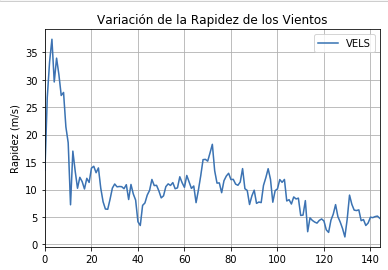
\includegraphics[width=0.5\textwidth]{ll.png}
\end{figure}

\newpage

Aqui podemos notar como es la variacion de la rapidez de los vientos en la ciudad de mexicali|, ahora mostraremos una grafica de variacion de la temperatura con la humedad relativa, aqui veremos como actuan estas dos variables con respecto una de la otra:
\begin{figure}[h]
\centering
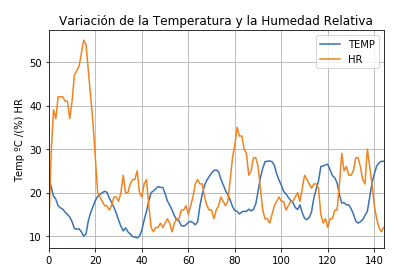
\includegraphics[width=0.5\textwidth]{ee.png}
\end{figure}

Aqui podemos ver que conforme la temperatura aumenta, la humedad relativa disminuye y viceversa. Ahora ¿como sera la variacion de la temperatura conforme transcurre el tiempo?, aqui lo podemos apreciar:
\begin{figure}[h]
\centering
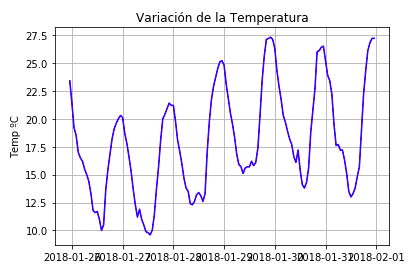
\includegraphics[width=0.5\textwidth]{ff.png}
\end{figure}

Asi nos damos cuenta de que la temperatura va variando conforme el tiempo transcurre, lo cual es normal, dado que pasando el tiempo el clima puede cambiar, junto con la temperatura.
\newpage

Ahora veremos como son la velocidad de los vientos contra la rapidez de las rafagas, y veremos su comportamiento:

\begin{figure}[h]
\centering
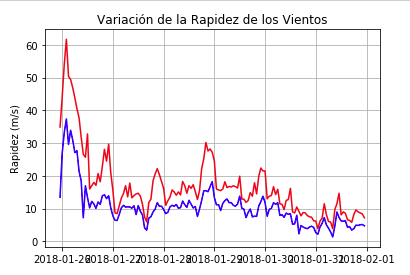
\includegraphics[width=0.5\textwidth]{gg.png}
\end{figure}

Por ultimo veremos como son la variacion de la dirreccion de los vientos que veremos que se mantiene mas o menos constante:

\begin{figure}[h]
\centering
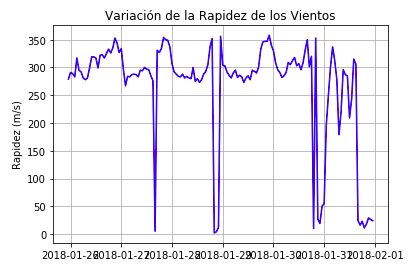
\includegraphics[width=0.5\textwidth]{vv.png}
\end{figure}

\newpage

\title{Apéndice}

\begin{itemize}
\item \textbf{¿cual es tu primera impresion de jupyter notebook?}
Me parece un entorno sencillo de trabajar una vez que se domina el lenguaje de programacion phyton.

\item \textbf{¿Se te dificultó leer código en Python?}
Al principio fue un pococ dificil por lo que necesite investigar y pedir ayuda.

\item \textbf{¿En base a tu experiencia de programación en Fortran, que te parece el entorno de trabajar en Python?}
Mucho mas sencillo que fortran

\item \textbf{A diferencia de Fortran, ahora se producen las gráficas utilizando la biblioteca Matplotlib. ¿Cómo fue tu experiencia?}
Me parecio sencillo una vez que practicas los comandos pde phyton para poder graficar.

\item \textbf{En general, ¿qué te pereció el entorno de trabajo en Python? }
Me parecio un entorno muy comodo y eficiente para poder trabajar en proyectos.

\item \textbf{¿Qué opinas de la actividad? ¿Estuvo compleja? ¿Mucho material nuevo? ¿Que le faltó o que le sobró? ¿Qué modificarías para mejorar? }
Pues creo que lo dificil sera aprender para que funcionan los diversos comandos de phyton, pero eso se hara con la practica, pienso que fue una actividad muy padre.

\item \textbf{¿Comentarios adicionales que desees compartir? }
Ninguno
\end{itemize}


\end{document}



